\documentclass[12pt]{article}
\usepackage[utf8]{inputenc}
\usepackage[russian]{babel}
\usepackage{mathrsfs}
\usepackage{amssymb}
\usepackage{amsmath}
\usepackage{graphicx}

\graphicspath{{pictures/}}
\DeclareGraphicsExtensions{.pdf,.png,.jpg}

\textheight=24cm
\textwidth=16cm
\oddsidemargin=0pt
\topmargin=-1.5cm
\parindent=24pt
\parskip=0pt
\tolerance=2000
\flushbottom

\newtheorem{Th}{Теорема}
\newtheorem{Def}{Определение}
\newtheorem{Lem}{Лемма}
\newtheorem{St}{Утверждение}
\newtheorem{Ex}{Пример}

\newenvironment{Proof}{\par\noindent{\bf Доказательство}}{$\blacksquare$} 
\newenvironment{Wtf}{
\includegraphics[height=5mm]{ping}}{}
\newenvironment{Why}{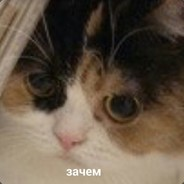
\includegraphics[height= 5mm]{cat}}{}

\numberwithin{Th}{section}
\numberwithin{Def}{section}
\numberwithin{Lem}{section}
\numberwithin{St}{section}
\numberwithin{equation}{section}
\counterwithin*{section}{part}

\newcommand\Set[2]{\left\{ #1 | #2 \right\}}
\newcommand\Pro{\mathbb{P}}
\newcommand\Ev{\mathscr{A}}

\begin{document}
\tableofcontents
\newpage

\part{Теория вероятности}
\newpage

\section{Вероятностное пространство}
\qquad Методы теории вероятности работают в ситуациях, называемых стохастическими. Для них характерны три свойства:
\begin{enumerate}
	\item Непредсказуемость 
	\item Воспроизводимость 
	\item Устойчивость частот
\end{enumerate}

Для описания стохастических ситуаций ситуаций необходимо определить функцию вероятности. Её область определения назывется множеством событий.
В свою очередь событие (такое как, например, выпадание чётного числа на кубике) могут являться совокупностью неких более простых событий, описывающих стохастическую ситуацию (число, выпавшее на кубике). Последнее множество называется множетсвом элементарных исходов и обозначается $\Omega$.  

Множество событий, обозначаемое $\Ev$, должно обладать следующими интуитивными свойствами:
\begin{enumerate}
	\item Отрицание события есть событие (если <<пойдет дождь>> событие, то <<не пойдет дождь>> также событие)
	\item Объединение событий есть событие (<<пойдет дождь>> или <<пойдет снег>>)
	\item Все множество элементарных исходов является событие (<<Что-нибудь да произойдет>>)
\end{enumerate}

Формализуя эти свойства, получаем определение алгебры.
\begin{Def}
Семейство $\Ev$ подмножеств множества $\Omega$  называется \\ \underline{алгеброй}, если 
\begin{enumerate}
	\item $\forall A \in \Ev, B\in \Ev \Rightarrow A \bigcup B \in \Ev$
	\item $\forall A \in \Ev \Rightarrow \overline{A} \in \Ev$
	\item $\Omega \in \Ev$
\end{enumerate}
\end{Def}

Из аксиом алгебры и формулы $A\bigcap B = \overline{\overline{A} \bigcup \overline {B}}$ следует, что пересечений событий явялется событием.

Наименьшей возможной алгеброй является $\left\{ \Omega, \varnothing \right\}$

\begin{Def}
Семейство $\Ev$ подмножеств множества $\Omega$  называется \\ \underline{$\sigma$-алгеброй}, если 
\begin{enumerate}
	\item $\forall A_1, \dots, A_n, \ldots \in \Ev \Rightarrow \bigcup\limits_{i=1}^{\infty} A_i \in \Ev$
	\item $\forall A \in \Ev \Rightarrow \overline{A} \in \Ev$
	\item $\Omega \in \Ev$
\end{enumerate}
\end{Def}

\begin{Def}
Пусть $\mathscr{K}$ - класс подмножеств $\Omega$. $\sigma$-алгебра $\sigma (\mathscr{K})$,\\ \underline{ порожденная классом $\mathscr{K}$} --- наименьшая $\sigma$-алгебра, 
содержащая $\mathscr{K}$
\end{Def}

$\sigma$-алгебра является более узким понятием, нежели алгебра, то есть любая $\sigma$-алгебра является алгеброй, а обратное, вообще говоря, неверно. Примером 
может послужить $\sigma$-алгебра, порожденная множеством отрезков $[a, b] \subseteq [0, 1]$ таких, что $a, b \in \mathbb{Q}$.

\begin{Def}
Пара $(\Omega, \Ev)$ называется \underline{измеримым пространством}, если $\Ev$ является $\sigma$-алгеброй. Если же $\Ev$ - алгебра, то  $(\Omega, \Ev)$ --- \underline{измеримое пространство} \underline{ в широком смысле}.
\end{Def}

\begin{Def}
\underline{Вероятностью} называется функция $\Pro \colon \Ev\rightarrow \mathscr{R}_+$, удовлетворяющая свойстам
\begin{enumerate}
	\item $\forall A \in \Ev \quad \Pro (A) \ge 0$
	\item $\forall A_1, \dots, A_n, \ldots \in \Ev \quad A_i \bigcap A_j  = \varnothing\  (i \not= j)  \Rightarrow \Pro (\bigcup\limits_{i=1}^{\infty} A_i) = \sum\limits_{i = 1}^{\infty} A_i$
	\item $\Pro (\Omega) = 1$
\end{enumerate}
\end{Def}

\begin{Def}
\underline{Вероятностным пространством} $(\Omega, \Ev, \Pro)$ называется измеримое пространство $(\Omega, \Ev)$, снабженное вероятностью $\Pro$.
\end{Def}
\begin{Wtf}
Кому вообще нужна $\sigma$-алгебра событий, и зачем весь этот огород, если можно рассматривать множество всех подмножеств множества $\Omega$? Когда-то кто-то доказал, что в случае очень большого множества элементарных исходов, например, континуального, множество $2^{\Omega}$ будет иметь такую крокодильски большую мощность, что вся теория сломается. Таким образом, алгебры нужны для того, чтобы вероятность имела хорошую область определения.
\end{Wtf}

\paragraph{Свойства вероятности}
\begin{enumerate}
	\item $\Pro (\varnothing) = 0$ 
	\item $\Pro (\overline{A}) = 1 - \Pro (A)$
	\item $B \subseteq A \quad \Rightarrow \Pro (A) \le \Pro (B)$
	\item $\Pro (A) \le 1$
	\item $\Pro (A \bigcup B) = \Pro (A) + \Pro (B) - \Pro (AB)$ 
	\item $\Pro (A \bigcup B) \le \Pro (A) + \Pro (B)$ 
	\item $\Pro (\bigcup\limits_{i=1}^{n} A_i) = \sum\limits_{k=1}^{n} \sum\limits_{i_1<\dots <i_k} (-1)^{k+1} \Pro(A_{i_1}A_{i_2}\ldots A_{i_k})$
	\item $\Pro (\bigcap\limits_{i=1}^{n} A_i) \ge 1 - \sum\limits_{i=1}^{n} \Pro (\overline{A_i})$ - неравенство Бонферрони
\end{enumerate}

Второй пункт в определении вероятностной меры нельзя заменить аналогичным с конечными объединением и суммой. Однако если добавить к данному требованию так 
называемое свойство непрерывности вероятностной меры, т.е $$\forall B_1, B_2, \ldots \in \Ev \quad B_{n+1} \subseteq B_n \Rightarrow \lim_{n \to \infty} \Pro(B_n) = \Pro(B)$$, то они вместе будут эквивалентны 2. из определения вероятности.

\begin{St}
$\forall A_1, \dots, A_n, \ldots \in \Ev \quad A_i \bigcap A_j  = \varnothing\  (i \not= j)  \Rightarrow \Pro (\bigcup\limits_{i=1}^{\infty} A_i) = \sum\limits_{i = 1}^{\infty} A_i
\Leftrightarrow ( \forall A_1, \dots, A_n \in \Ev \quad A_i \bigcap A_j  = \varnothing\  (i \not= j)  \Rightarrow \Pro (\bigcup\limits_{i=1}^{n} A_i) = \sum\limits_{i = 1}^{n} A_i)  \land  (\forall B_1, B_2, \ldots \in \Ev \quad B_{n+1} \subseteq B_n \Rightarrow \lim\limits_{n \to \infty} \Pro(B_n) = \Pro(B))$
\end{St}
\begin{Proof}
\\ $\Rightarrow$\\
Обозначим $C_n = B_n \setminus B_n+1$. Множества $B, C_1, C_2, \ldots$ не имеют общих точек.\\
$\forall n \quad B_n =  \bigcup\limits_{k=n}^{n} C_k \bigcup B$. Тогда $\Pro(B_1) = \Pro(B) + \sum\limits_{k=1}^{\infty} \Pro(C_k)$. Отсюда следует, что ряд в правой части сходится, так как имеет конечную сумму.
$\Pro(B_n) = \Pro(B) + \sum\limits_{k=n}^{\infty} \Pro(C_k)$. При $n \to \infty$ сумма ряда стремится к нулю как остаточный член ряда из предыдущего выражения.
В предельном переходе получаем свойство непрерывности.
\\ $\Leftarrow$\\
Рассмотрим произвольный набор $A_1, A_2, \ldots \in \Ev \quad A_iA_j = \varnothing$.\\
$\Pro(\bigcup\limits_{i=1}^{\infty} A_i) = \Pro(\bigcup\limits_{i=1}^{n} A_i) + \Pro(\bigcup\limits_{i=n + 1}^{\infty} A_i) =\sum\limits_{i = 1}^{n} \Pro(A_i) +  
\Pro(\bigcup\limits_{i=n + 1}^{\infty} A_i) $.\\
 Обозначим $B_n = \bigcup\limits_{i=n + 1}^{\infty} A_i,\quad B_{n+1} \subseteq B_n \quad \forall n,\quad \bigcap\limits_{n=1}^{\infty} B_n= \varnothing$ \\
$\sum\limits_{i=1}^{\infty} \Pro(A_i) = \lim\limits_{n \to \infty} (\Pro(\bigcup\limits_{i=1}^{\infty} A_i) - \Pro(B_n)) = \Pro(\bigcup\limits_{i=1}^{\infty} A_i) - \lim\limits_{n \to \infty} \Pro(B_n) = \Pro(\bigcup\limits_{i=1}^{\infty} A_i)$
\end{Proof}

\begin{Th}[Каратеодори]
Пусть $(\Omega, \Ev)$ --- измеримое пространство в широком смысле, а некоторая функция $\Pro$ обладает свойствами вероятностной меры.Тогда на измеримом пространстве
$(\Omega, \sigma(\Ev))\  \exists !\  \Pro' \colon \forall A \in \Ev \quad \Pro(A) = \Pro'(A)$
\end{Th}
\begin{Proof}
отсутсвует
\end{Proof}\\\\
\begin{Why}
Зачем это нужно? Теорема Каратеодори говорит о том, что любую вероятностную меру, заданную на алгебре, можно однозначно продолжить на $\sigma$-алгебру,
то есть расширить область ее определения. При этом значения функции на алгебре не изменятся. Теорема будет использоваться при определении интеграла Лебега.
\end{Why}
\end{document}